\documentclass{mcmthesis}

\mcmsetup{CTeX = true,   % 使用 CTeX 套装时,设置为 true
        tcn = 2215432, problem = E,
        sheet = true, titleinsheet = true, keywordsinsheet = true,
        titlepage = false, abstract = false}
\geometry{left=0.75in,right=0.75in,top=1in,bottom=1in}
\numberwithin{figure}{section}
\numberwithin{table}{section}
\numberwithin{equation}{section}
\usepackage{newtxtext}
\usepackage{lipsum}
\usepackage{palatino}
\usepackage{hyperref}
\usepackage{booktabs}
\usepackage{subfigure}
\usepackage{graphicx}
\usepackage{pythonhighlight}
\usepackage{indentfirst}%首段自动缩进
\usepackage{colortbl}
\usepackage{apacite}
\usepackage{natbib}
\usepackage{tablefootnote}
\usepackage{multicol}
%算法四部曲↓
\usepackage{algorithm}
\usepackage{algpseudocode}
\usepackage{amsmath}
\usepackage{algorithmicx}
% \usepackage{threeparttable}

\setlength{\parindent}{2em}
\title{123}
\setlength{\headheight}{15pt}

\begin{document}
\renewcommand{\algorithmicrequire}{\textbf{Input:}}  % Use Input in the format of Algorithm
\renewcommand{\algorithmicensure}{\textbf{Output:}} % Use Output in the format of Algorithm
\begin{abstract}



\begin{keywords}
\end{keywords}
\end{abstract}
\maketitle

\tableofcontents
  \thispagestyle{empty}
  \newpage
  \setcounter{page}{1}
%%
%%Generate the Memorandum, if it's needed.
%\memoto{\LaTeX{}studio}
%\memofrom{Liam Huang}
%\memosubject{Happy \TeX{}ing!}
%\memodate{\today}
%%\logo{\LARGE I'm pretending to be a LOGO!}
%\begin{memo}[Memorandum]
%  \lipsum[1-3]
%\end{memo}

\section{Introduction}

\subsection{Problem Restatement}
Considering that the carbon dioxide can be sequestered in both forests 
and wooden products, it's reasonable that more carbon will be stored by forests with the 
appropriate combination of the regrowth of younger forests and the wooden products.
Thus, forest managers are ought to deliberate about the balance between the value of forests 
as living tress to grow and absorb the carbon and the value of forests harvested as wooden products.
What's more, the forest managers should not only consider the factors about forests such as 
type and age of forests, geography, topography, and benefits and lifespan of forest products,
but also the conservation and diversity of wild species, recreational uses and cultural considerations.
\begin{enumerate}
    \item [1.] Design a carbon sequestration model to calculate the amount of carbon dioxide 
    sequestered by a forest and its products, which also determines what kind of manage plan is
    most efficient at sequestering carbon.
    \item [2.] Develop a decision model consisting of various ways that forests are valued (including
    carbon sequestration) for forest managers to understand the best use of a forest. Consider 
    the following questions. What is the scope of the management plan that your decision model might suggest?
    Are there any conditions that the forests should not be harvested?
    Whether there is a transition point between management plans applicable to all forests?
    How can the characteristics of a particular forest and its location be used 
    to determine transition points between management plans?
    \item [3.] Apply your models to various forests. Identify a forest that your decision model 
    would suggest the inclusion of harvesting in its management plan.
    How much carbon dioxide can be sequestered by this forest and its products in 100 years?
    What kind of forest management plan should be carried out for this forest? Why it's best?
    The best management plan is assumed to include a harvest interval of 10 
    years longer than current forest practices discussing strategies for transitioning 
    from existing to new schedules in a manner sensitive to the needs of forest managers 
    and all those who use forests.

    \item [4.] Some people think that we should never cut down any trees, but you've
    determined the forest which includes harvest in its management. Write a one-to-two-page
    non-technical newspaper articles to explain why your analysis including in the 
    management of the forest logging, rather than it remaining the same. Finally, your ariticle 
    should convince local community that it's the best decision for their forest.
\end{enumerate}

\subsection{Overview of Our Work}




\section{Assumptions and Justifications}
These are necessary assumptions for simplifying the model.
\begin{enumerate}
  \item [1.] 
\end{enumerate}


\section{Notations}

\renewcommand\arraystretch{1.5}

\begin{table}[htpb!]
  \centering
  \caption{Notation Descriptions}
  \begin{tabular}{m{2.5cm}<{\centering}|m{12.5cm}<{\centering}}
  \toprule[1.5pt]
  \textbf{Symbol} & \textbf{Definition} \\ \hline
  $ \rm{DBH} $ & Diameter at Breast Height \\
  $ \beta_b $ & Conversion factor of coniferous trees\\
  $\beta_c$ & Conversion factor of broad leaf trees\\
  $ n $ & Total iteration years\\
  $ \lambda $ & Harvest rate\\
  $ M $ & Sequestered carbon mass in wooden products \\
  $ \rm{CarbonMass_f} $ & Sequestered carbon mass in forests \\
  $ \phi $ & Proportion in total product\\
  $ s $ & Scrap rate\\
  $ m $ & Decomposition rate \\

  \bottomrule[1.5pt]
  \end{tabular}
\end{table}

\newpage

% 标题可能需要修改
\section{Binary Volume and Logistic based Carbon Sequestration Model}

In order to clearly demonstrate the amount of carbon sequestered by forests and their
products, we decide to consider the trunk volume of living trees as an estimation of 
total Volume of trees that are able to store carbon \citep{WangYan}. 
\par
For the living trees, we apply Binary Timber Volume Regression model \citep{LuoQingbang} 
to depict their growth as shown in Algorithm \ref{Binary Volume Algo}. 
It is significant
to point out that $ \beta_b $ and $ \beta_c $ are two \textbf{Conversion Factors} from
Timber Volume to Carbon Mass sequestered. Besides, the mass of carbon sequestered in
soil and leaves can be deemed as a constant which merely depends on the area
of coniferous and broad-leaved forests \citep{YanDeren2011}. 
\par
As for the wooden products, we consider $ w $ kinds of wooden products, each kind,
which decomposes at the rate of $ m_i (i = 1,\cdots, w) $, accounts for $ \phi_i$ 
of the total product mass \citep{2006Forest}. Note that the \textbf{harvest rate} $ \lambda $ and the product
proportion $ \phi $ are flexible regarding the circumstances, which are also 
the core of our forest management. What's more, we hold the view that 
the volume of wooden products derive from the volume of harvested trees with a certain
\textbf{Scrap Rate} $ s $. The complete idea is shown in Algorithm \ref{Product Algo}.
\par
\begin{figure}[ht]
  \begin{minipage}[htbp]{0.42\linewidth}
    The Scrap Rate is determined as following descriptions, which is also shown 
    in Figure \ref{RoundWood} on the right. There are two 
    manufacturing methods of Round Wood harvested from the forests. 
    \par
    One way is to trim the wood neatly into slabs in different shapes so that they can
    occupy most of the volume of the wood, which will be processed into softwood plywood, 
    panels and board. Meanwhile, the scrap will be manufactured into miscellaneous 
    products. It can approach the utilization rate of 81.3\%.
    \par
    The other kind of craft is to separate the bark and turn it into paper, and 
    the separated log can be processed into softwood and hardwood. The utilization 
    rate of this craft is able to reach almost 100\%.
  \end{minipage}
  \hfill
  \begin{minipage}[htbp]{0.5\linewidth}
    \begin{flushright}
      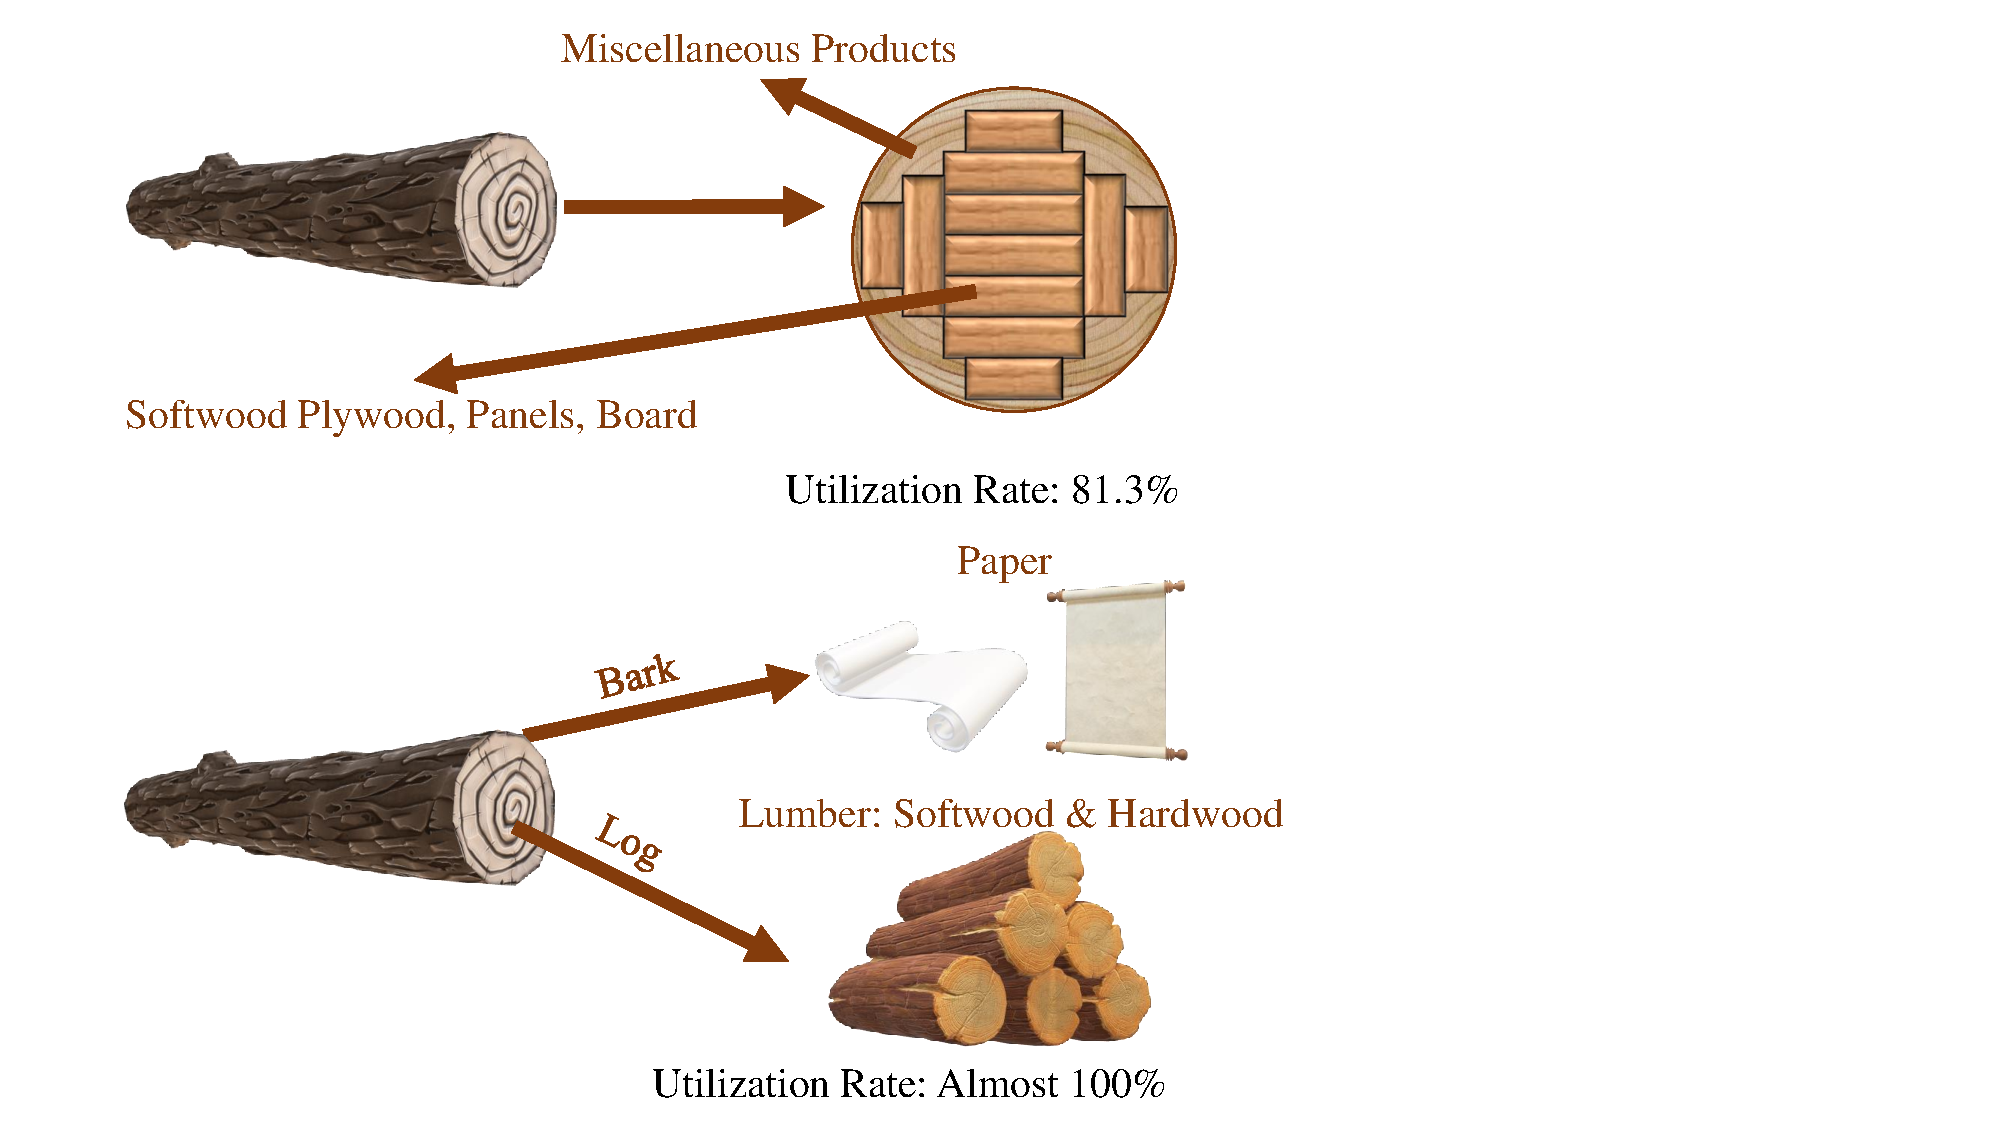
\includegraphics[width = 8.61cm]{code&pic/Roundwood cutting ways.pdf}
      \caption{Utilization Rate of Round Wood}\label{RoundWood}
    \end{flushright}
  \end{minipage}
  \end{figure}




\begin{algorithm}[htbp]
    \caption{Binary Timber Volume Regression of Carbon Prediction Algorithm}\label{Binary Volume Algo}
    \begin{algorithmic}[1]
      \Require
        Measurement of DBH, Height of tree ($ h $), conversion factor 
        $ \beta_c $  (coniferous) and $ \beta_b $ (broad leaf), Harvest rate $ \lambda(t) $, Carrying Capacity $ K $  
        \For{x in enumarate $ (\rm{DBH},h) $ }
        \For{k $ \gets 1$ to $ m $}
        $ P_k(x) = \frac{1}{2^kk!}\frac{d^k}{dx_k^k}(x^2-1)^k $
        \For{$ l \gets 1 $ to $m$ }

        \quad \quad Calculate $ \int_{-1}^{1}P_k(x)P_l(x)dx \gets $ Integral of Legendre Polynomials
        \If{$ k = l $}$ \int_{-1}^1P_k(x)P_l(x) = \frac{2x}{2i+1} $
        \Else $ \int_{-1}^1P_k(x)P_l(x) = 0 $   
        \EndIf 
        \EndFor
        \EndFor
        \EndFor
        
        \noindent Find $ (\rm{DBH}, h)^T $ to minimize  $ J = \int_a^b[f(\rm{DBH})+g(h)-2(x)]^2dx $
        \For{$ t \gets 1 $ to $ n $ }

        Regression of DBH and $ h $  

        $V_0 \gets$ Initiate

        $ V_t = a\rm{DBH}^bh^c\times Area\times \rm{Density}(\lambda, t)  $
        \EndFor

        \noindent$ Area = Area_b + Area_c $

        \noindent $ \rm{CarbonMass_f} $  $= (\beta_cV_c+\beta_bV_b)+9.6\times Area_c\times 
        \frac{\rm{Density}(\lambda,t)}{K}+3.4\times Area_b \times \frac{\rm{Density}(\lambda,t)}{K}+ 70\times Area$

        \Ensure
        Carbon Dioxide Quantity of Forest = $\frac{44}{12}\times\rm{CarbonMass_f}$ 
    \end{algorithmic}
  \end{algorithm}
  
  \begin{algorithm}[htbp]
    \caption{RBF Neural Network Fitting of wooden products for carbon sequestration Algorithm} \label{Product Algo}
    \begin{algorithmic}[1]
        \Require
            $ \phi $, $ s $, $ m $, $ w $ as kinds wooden products, Standardized CarbonMass and $ V $ in Algorithm1 
        \For{$ t\gets1 $ to n}
            \For{$ i\gets1 $ to hidden\_dim}

                $ y_0 \gets Initiate $ 

                $ \hat{y_t} = \hat{y_{t-1}} + \phi_{it}V_i(t) $
            
                $ c_i\gets $ Sample CarbonMass
            
                $ \sigma_i\gets $ Z-score Normalization

                $ V_i(t) = e^{-\frac{||t-c_i||^2}{2\sigma_i^2}} $
            \EndFor

            $ M_0\gets Initiate $ 

            \For{$ j\gets 1$ to $ w $}

            $ M_t = M_{t-1}+(1-s)\frac{\rm{Density}(\lambda, t-1)-\rm{Denstity}(\lambda,t)
            }{\rm{Density}(\lambda, t-1)}(\beta_cV_c(t-1)+\beta_bV_b(t-1))\times (\phi_j(t)m_j(t)) $ 
            \EndFor
        \EndFor
        \Ensure
        Carbon Dioxide Quantity of Wooden Products = $ \frac{44}{12} \times M_t$ 
    \end{algorithmic}
\end{algorithm}

We apply our model over a hypothetic forestry land with 10000 hectares, in which
the broad leaf trees takes one half and the other half is coniferous trees. Two
primary decision factors, which are harvest rate and product proportion,
are discussed by conducting sensitivity test. 
\par
The sensitivity test of Harvest Rate is conducted by calculating the Carbon Dioxide
sequestered by the living trees and the wooden products every 1\% of 
harvest rate from 1\% to 30\%, which can be seen in Figure \ref{Harvest Rate sensTest}.
\par
The sensitivity test of Product Proportion is carried out by determining the 
Carbon sequestered by wooden products under different types of product proportion
arrangement. The proportion of products with higher Decomposition Rate increases
from Type 1 to Type 5, which means in Type 5, most of the wood is consumed to manufacture
high Decomposition Rate products. The result is shown in Figure \ref{Product Proportion sensTest}.

\begin{figure}[htbp]
  \centering
  \subfigure[]{
  \centering
  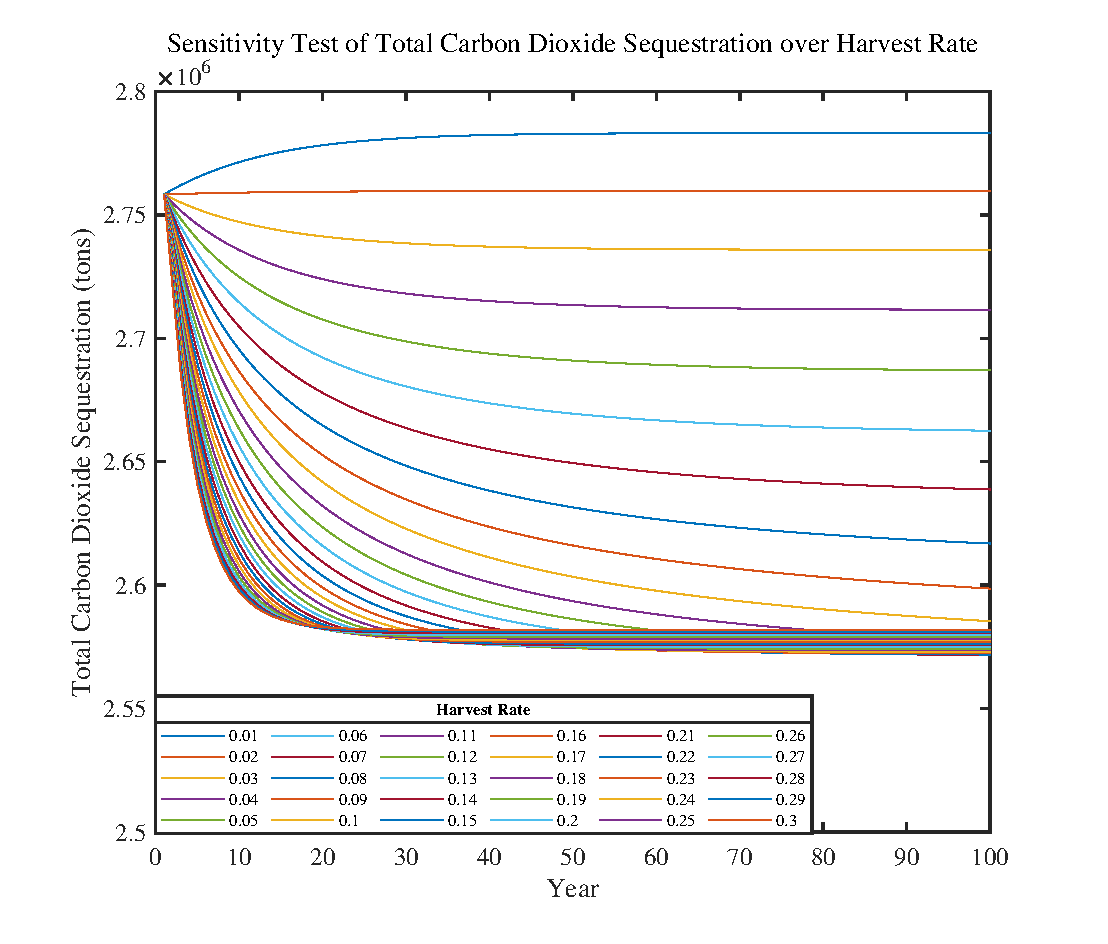
\includegraphics[width = 0.48\textwidth]{code&pic/HarvestRate.eps}\label{Harvest Rate sensTest}
  }
  \subfigure[]{
  \centering
  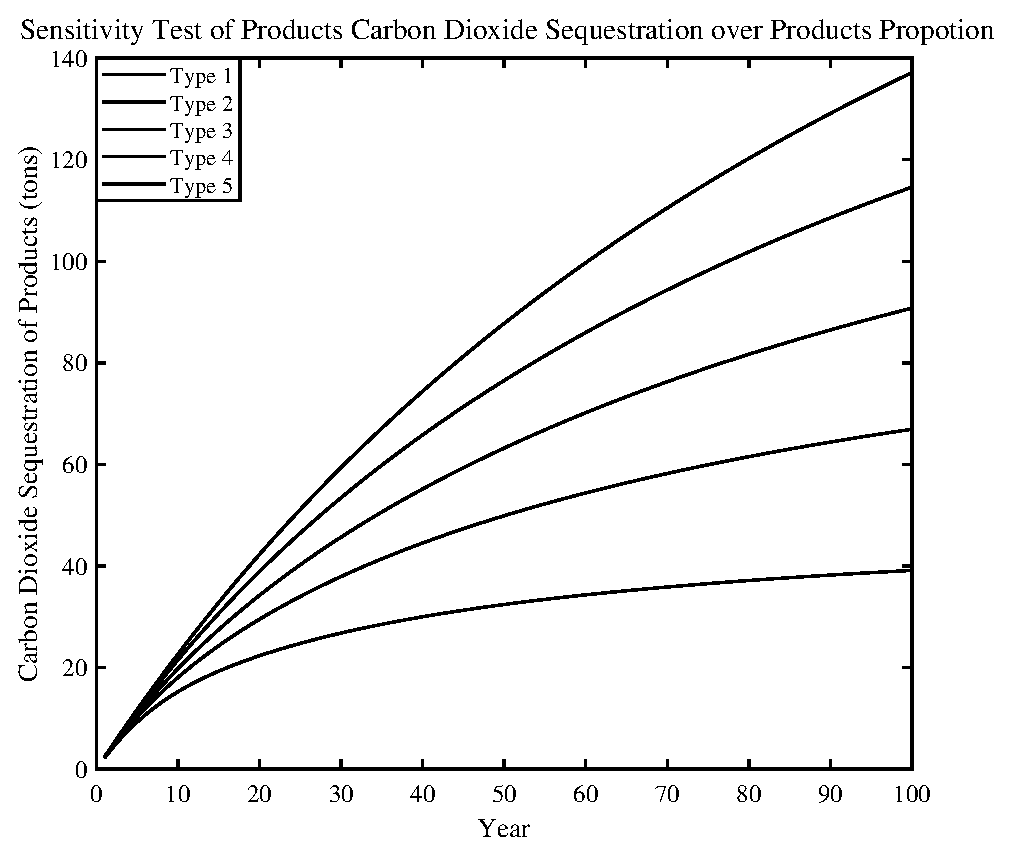
\includegraphics[width = 0.48\textwidth]{code&pic/proportion.eps}\label{Product Proportion sensTest}
  }

\caption{Results of sensitivity test of Harvest Rate and Product Proportion}
\end{figure}






\newpage

\subsection{Model III: Cellular Automata based Population Size Prediction}

Cellular automata (CA) is a kind of grid dynamics model with discrete time, 
space and state, and local spatial interaction and temporal causality, which 
has the ability to simulate the space-time evolution process of complex system.
\par
Unlike general dynamical models, cellular automata are not determined by strictly 
defined physical equations or functions, but are composed of rules constructed by 
a series of models. Any model that satisfies these rules can be regarded as a cellular 
automata model. Therefore, cellular automata is a general term for a class of models, 
or a method framework. Its characteristic is that time, space and state are discrete, 
each variable only takes a finite number of states, and its state change rules are local 
in time and space.
\par
The block diagram of a typical cellular automata is shown in Figure \ref{CA_Fig}, 
and the simulation result is shown in Figure \ref{CA_Result}, in which
we learn that the under the natural circumstances, the forestry population size
will reach and remain around 2100 per hectare. 



\begin{figure}[htbp]
  \centering
  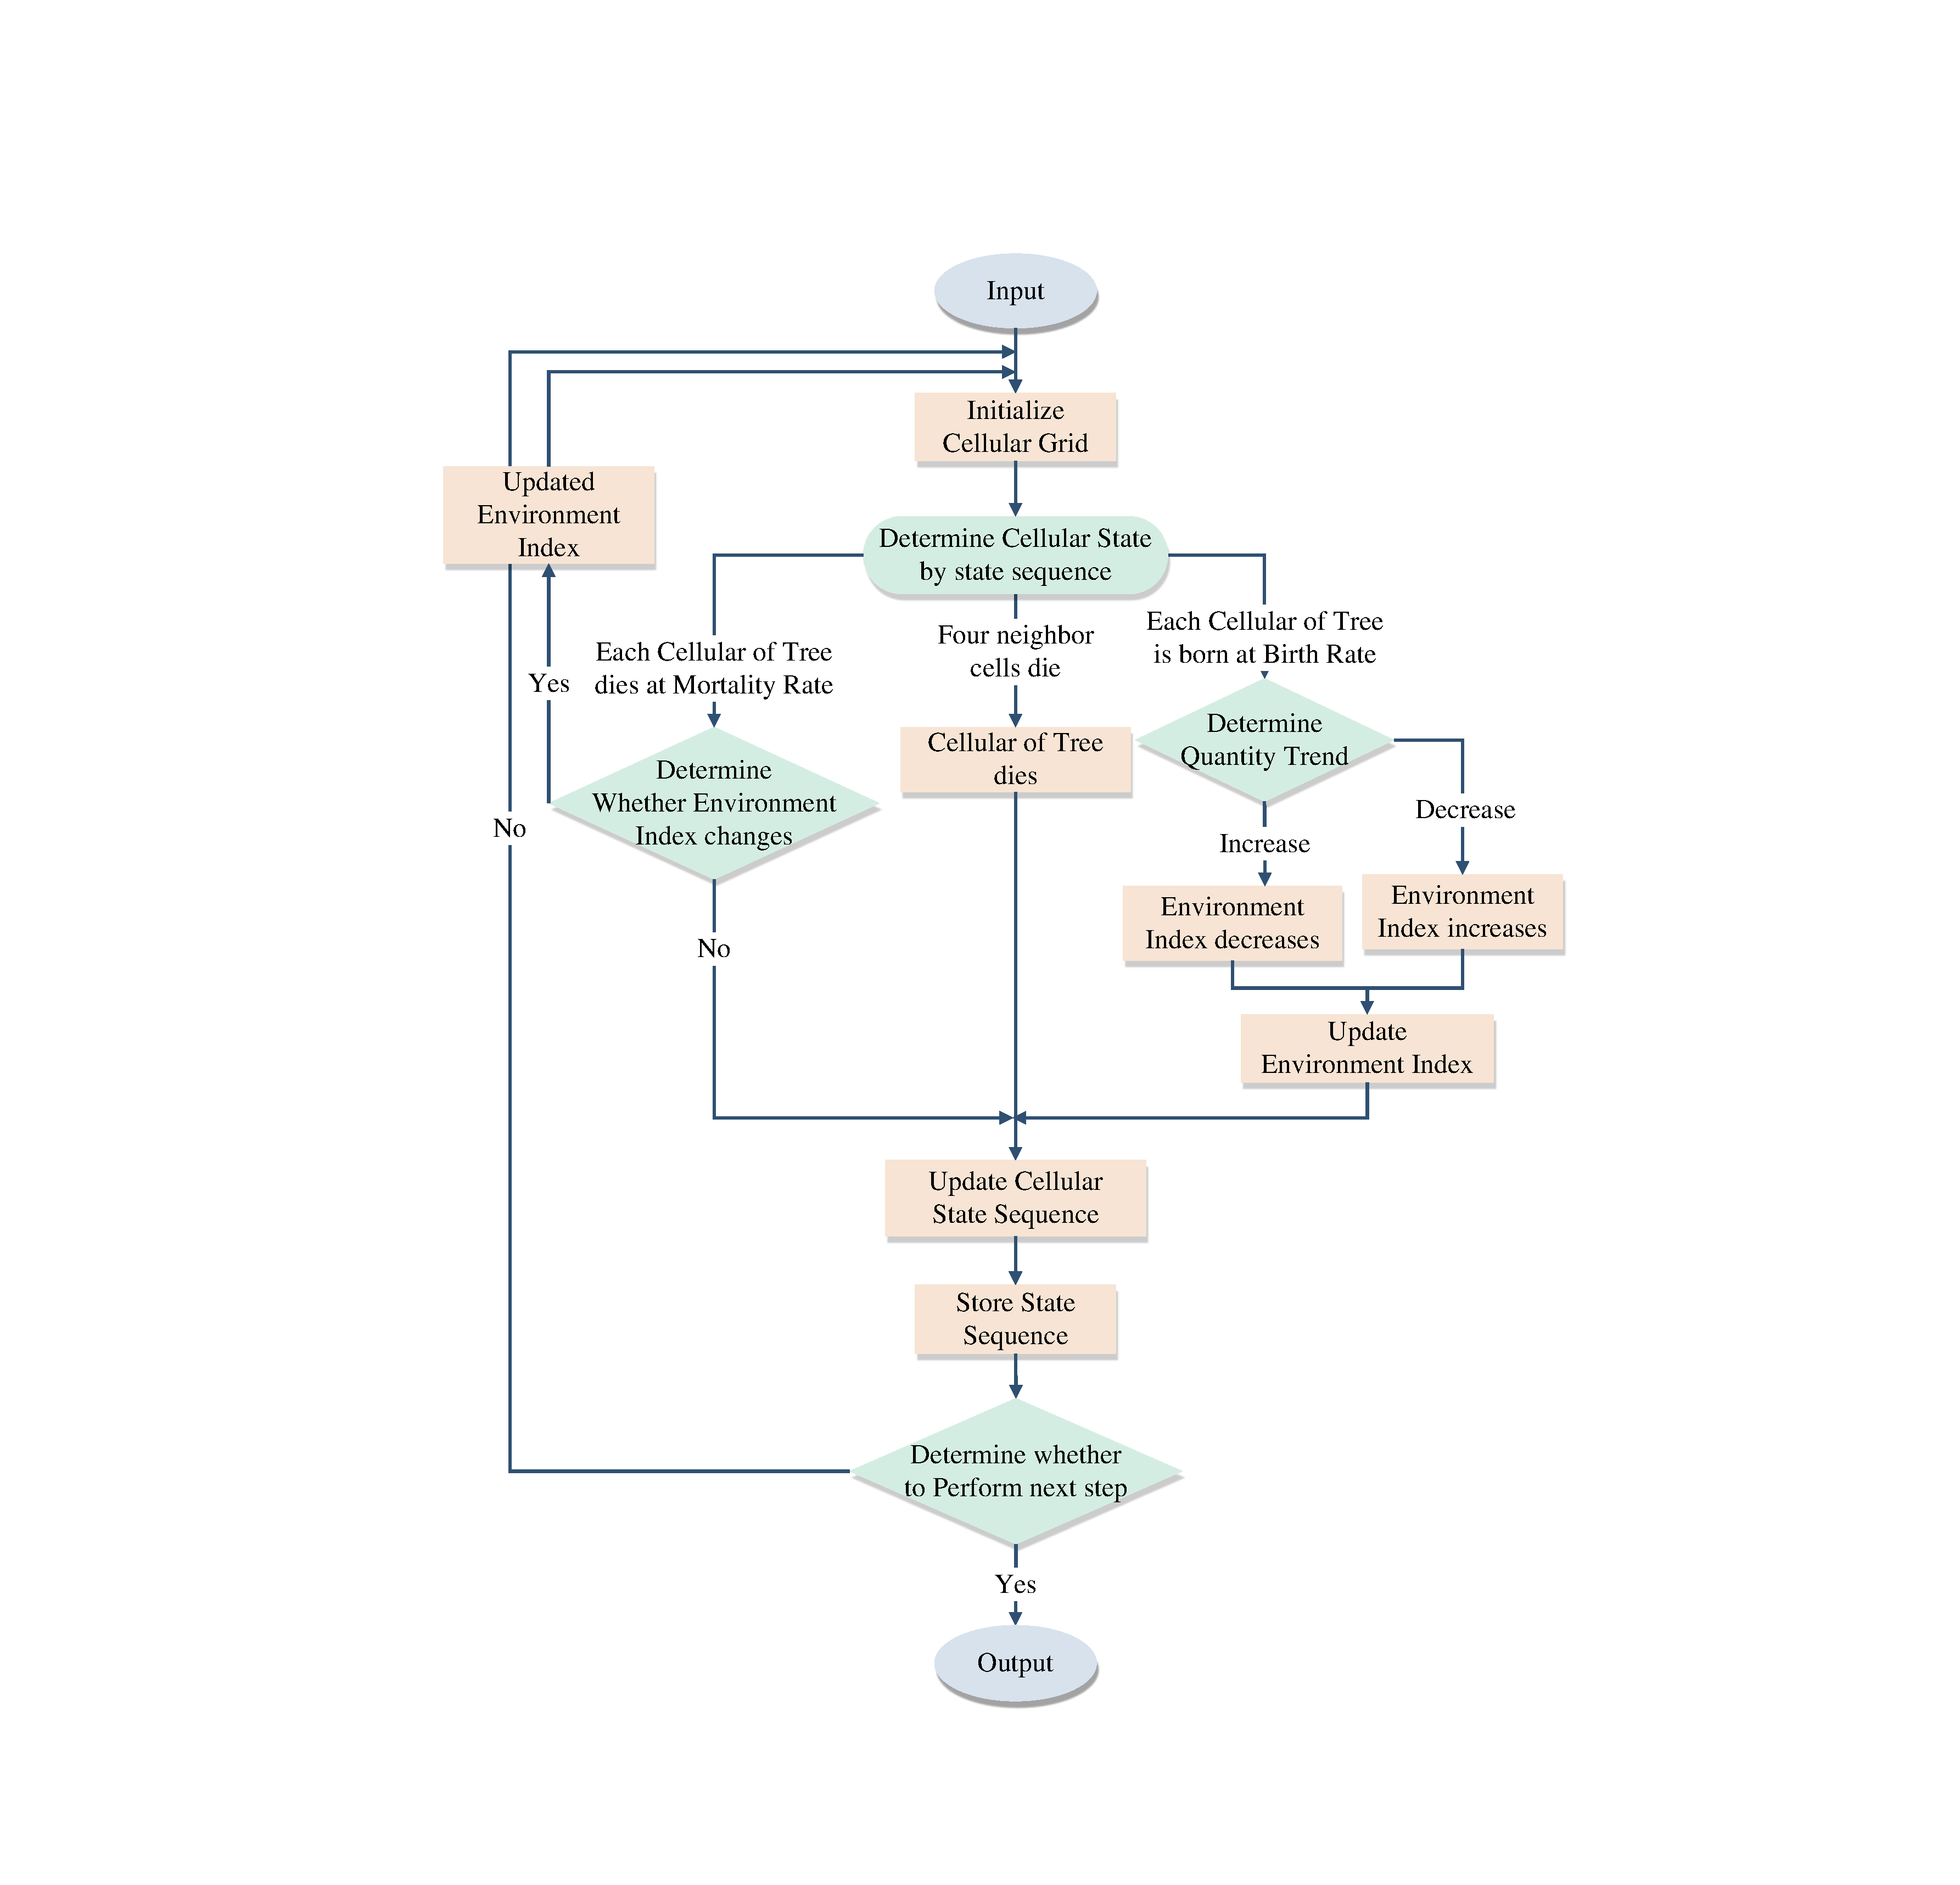
\includegraphics[width = 12cm]{code&pic/元胞自动机流程图.pdf}
  \caption{Block Diagram of typical Cellular Automata}\label{CA_Fig}
\end{figure}

\begin{figure}[t]
  \centering
  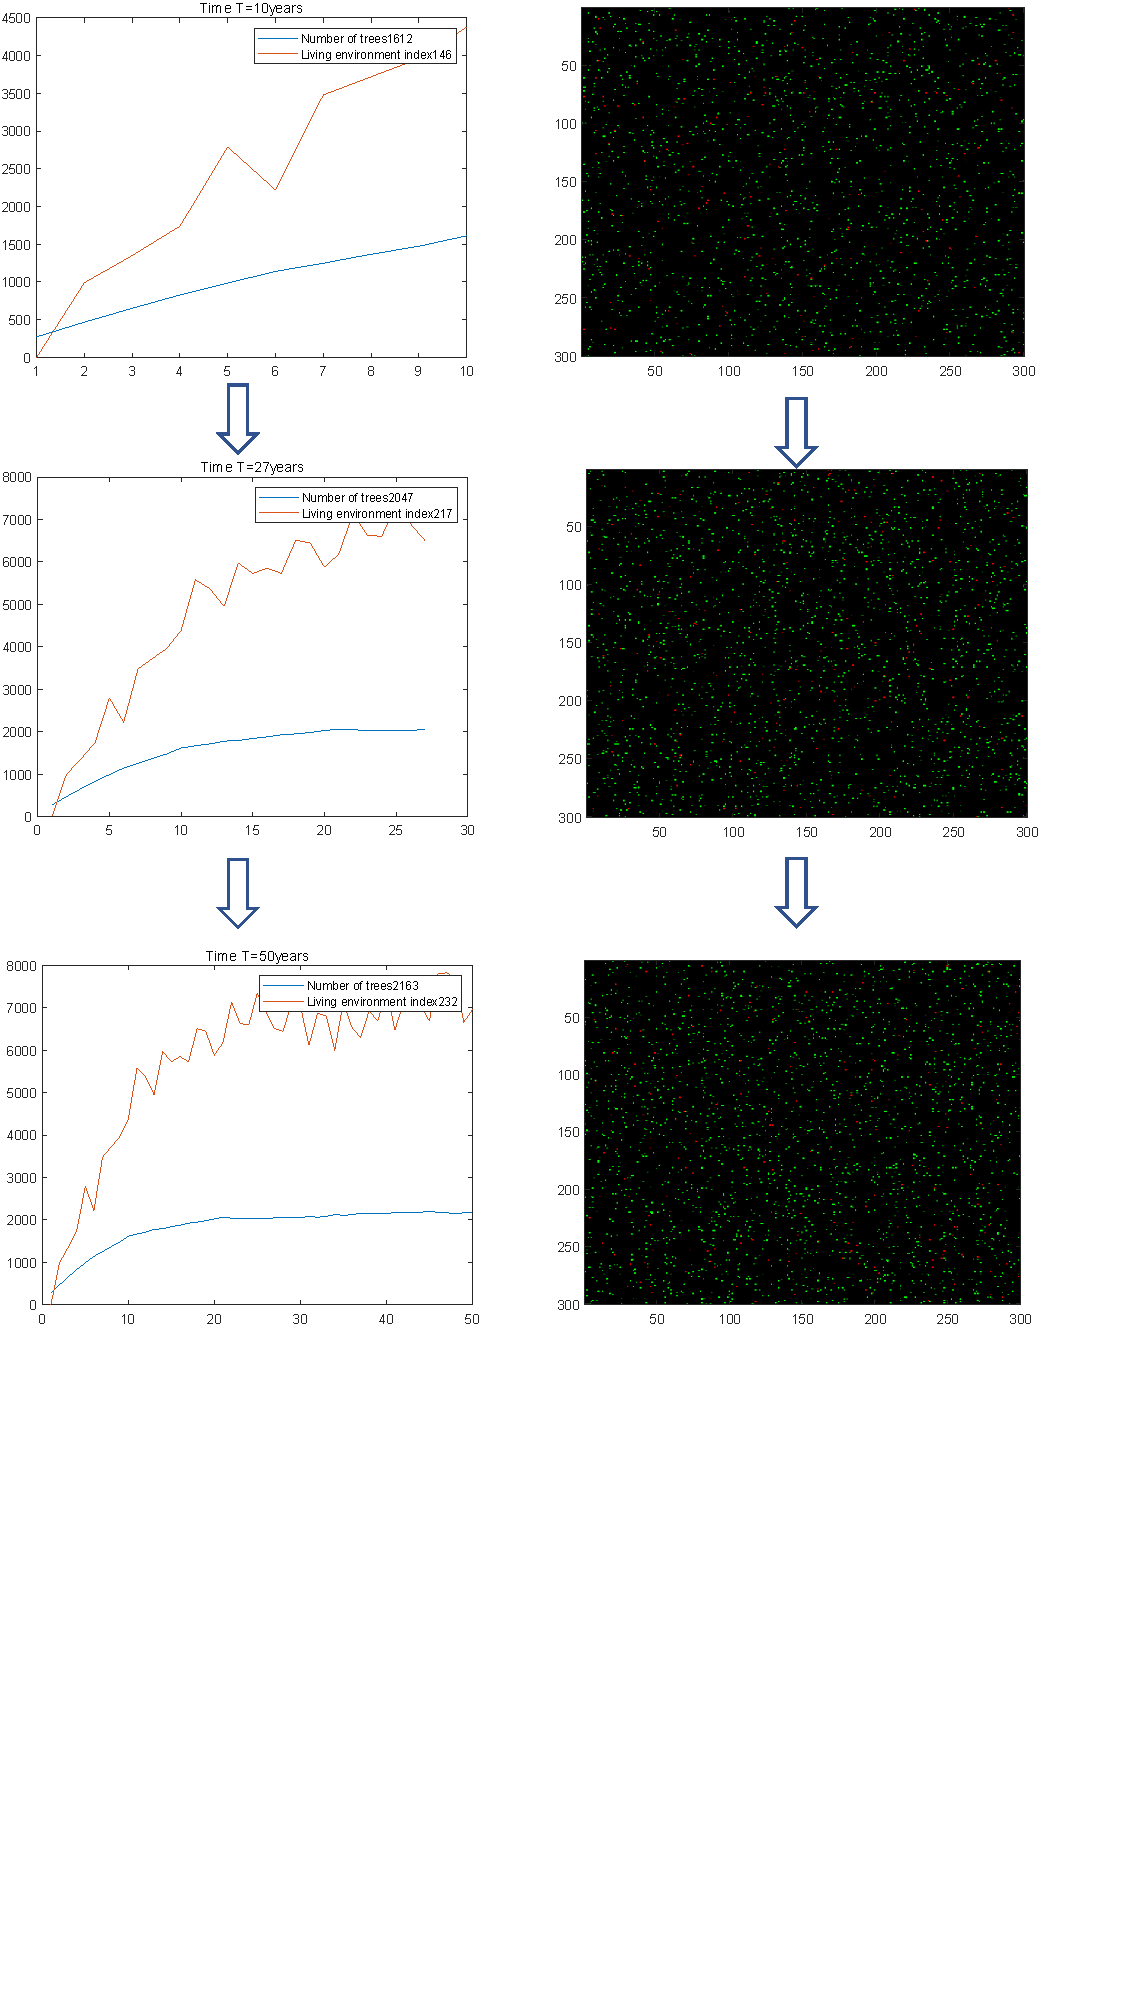
\includegraphics[width = 14cm]{code&pic/CA-pic.pdf}
  \caption{Result of Cellular Automation}\label{CA_Result}
\end{figure}




\section{Model II}
\begin{figure}[htbp]
  \centering
  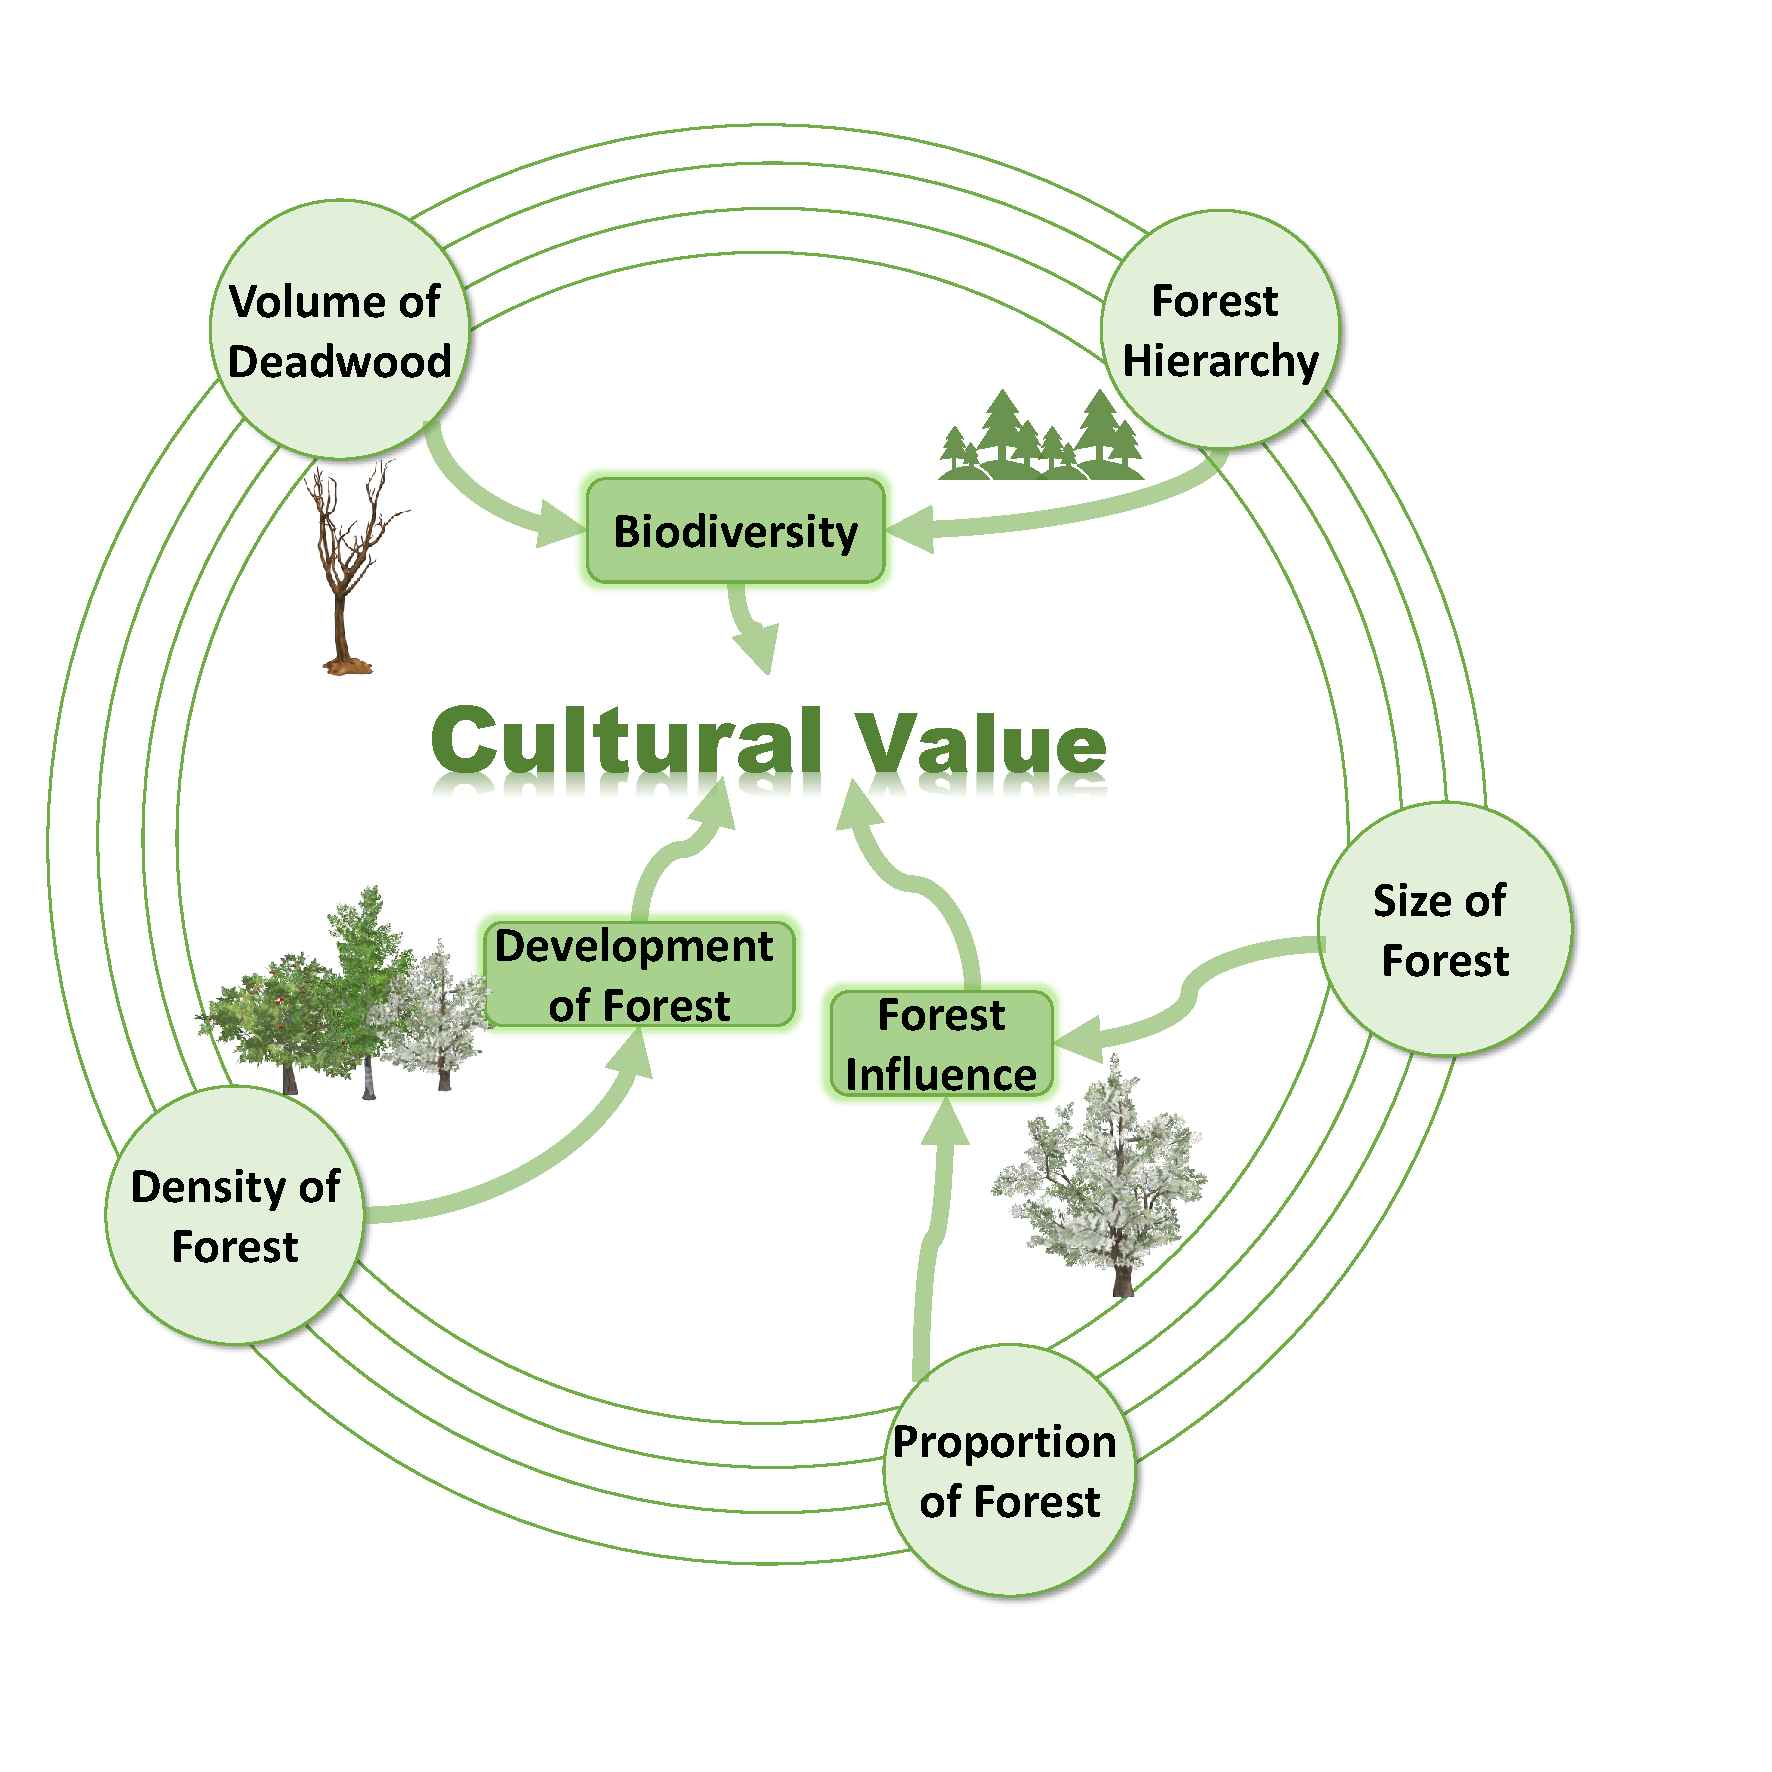
\includegraphics[width = 12cm]{code&pic/Model2.pdf}
  \caption{Influencing factors of Forest Culture Value}
\end{figure}

\begin{figure}[htbp]
  \centering
  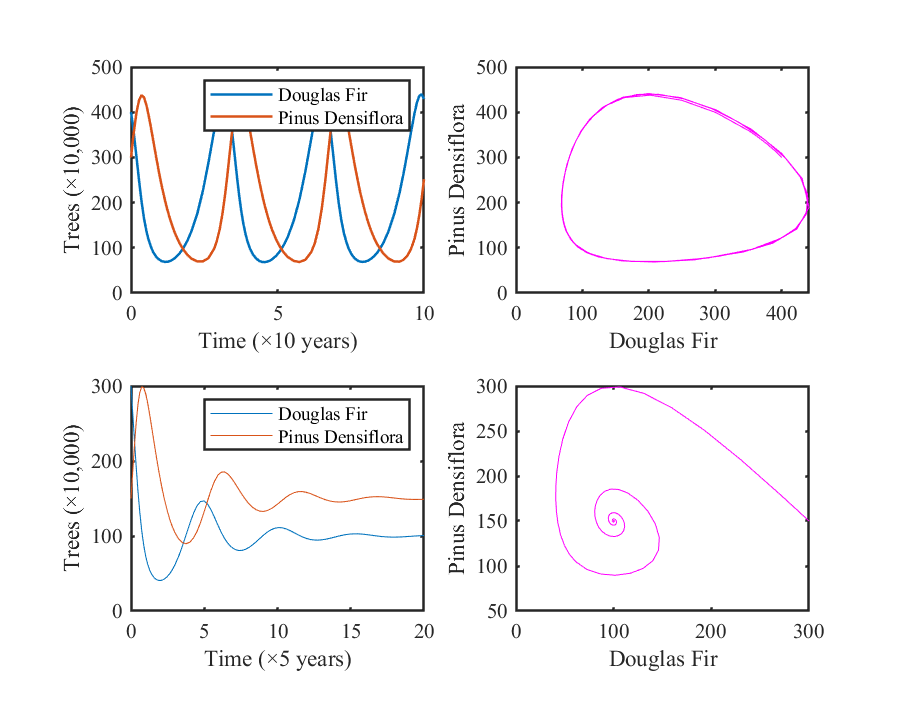
\includegraphics[width = 12cm]{code&pic/Interspecies.eps}
\end{figure}

\begin{figure}[htbp]
  \centering
  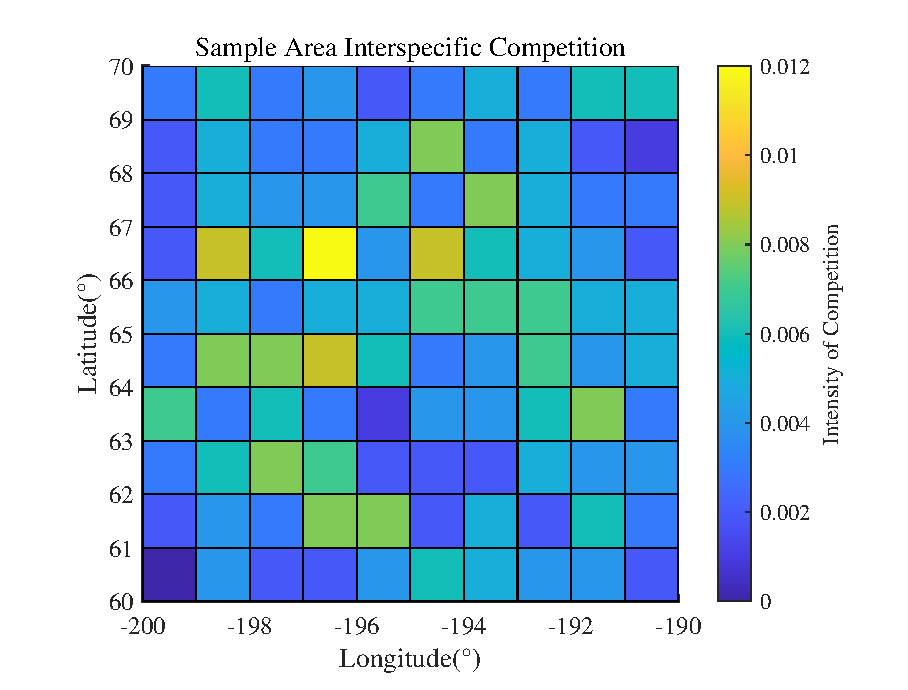
\includegraphics[width = 12cm]{code&pic/Interspecies-matrix.eps}
\end{figure}


\section{Sensitivity Test}
\begin{figure}[ht]
  \begin{minipage}[htbp]{0.4\linewidth}
    We assume that the density of the forest population follows the Logistic Model,
    and the \textbf{Carrying Capacity of the trees} is $ K $. From the Carbon Sequestration
    probability predicted on the right we can draw a reasonable conclusion that
    the Logistic Model will result into chaos after 3.6 rounds of harvests. 

  \end{minipage}
  \hfill
  \begin{minipage}[htbp]{0.55\linewidth}
    \begin{flushright}
      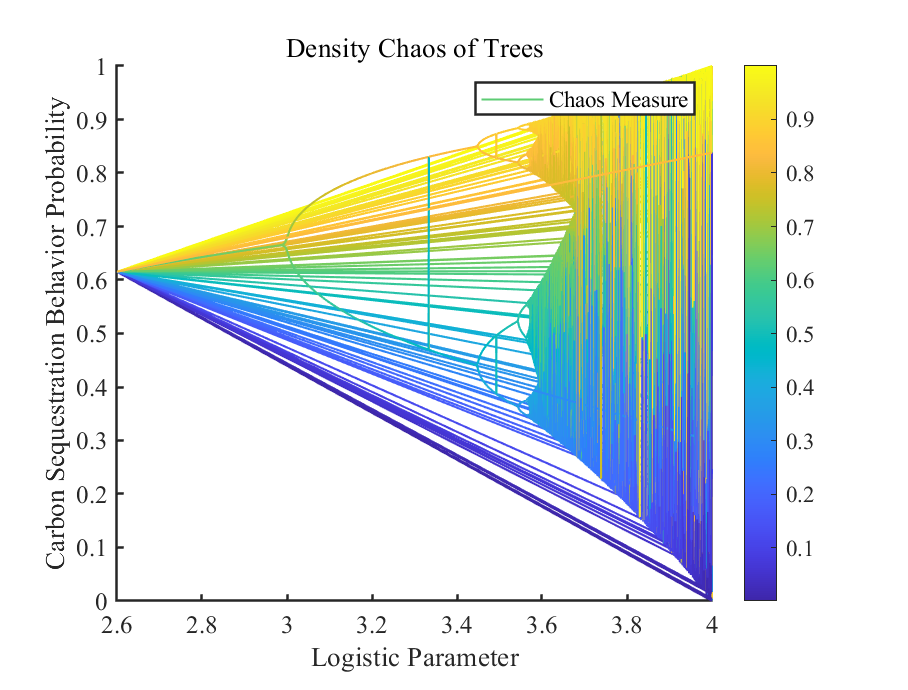
\includegraphics[width = 9cm]{code&pic/Logistic.eps}
    \end{flushright}
  \end{minipage}
\end{figure}
\section{Evaluation of Model}

\textbf{Strength:}


\section{Conclusions}



\newpage
\phantomsection\addcontentsline{toc}{section}{Policy Advice on Finless Porpoise Conservation}\tolerance=500
\memoto{Relavant Authorities}
\memofrom{MCM/ICM team 2215432}
\memodate{\today}

\begin{memo}[Policy Advice on Finless Porpoise Conservation]

  
\end{memo}




\newpage

%这一行是用来将Reference添加到目录的
\phantomsection\addcontentsline{toc}{section}{Refence}\tolerance=500

\bibliographystyle{apacite}
\bibliography{reference.bib}


\lhead{\small\sffamily \team}
% \rhead{\small\sffamily Page \thepage\ }

\begin{appendices}

% \textbf{\textcolor[rgb]{0.98,0.00,0.00}{Input python source:}}
% \lstinputlisting[language=python]{./codes/verhulst.py}


% \textbf{\textcolor[rgb]{0.98,0.00,0.00}{Input matlab source:}}
% \lstinputlisting[language=Matlab]{./codes/lagrange_main.m}


\end{appendices}


\end{document}

